% Fig. 1 and Fig. 2 of the paper merged into one figure, panels (a)-(d).
% Paste into the manuscript (revtex4-2, reprint). Needs in the preamble:
%   \usepackage{pgfplots} \pgfplotsset{compat=1.18}
% and the four panel_*.tex files next to the manuscript (or adjust the \input paths).
% The panels are drawn \columnwidth wide; inside this figure that width is set to a fraction of
% \textwidth so that two panels and their (a)-(d) labels fit the page. Font sizes do not change.
\begin{figure*}
  \centering
  \setlength{\columnwidth}{0.42\textwidth}%
  \pgfplotsset{every axis/.append style={ytick={0,0.2,0.4,0.6,0.8,1}}}%
  \begin{tabular}{@{}c@{\hspace{6mm}}c@{}}
    % generated by scripts/pkl_to_latex.py
% source PKL : uscan_v1_L6_Ne6_t1_mode-uniform_nmin2_solver-gcg_sz0_restarts10_iter200_kmax4_tol1em09_U1to20_N20-d03a74da789e.pkl
% scan type  : uscan
% state      : gs
% requires   : \usepackage{pgfplots} \pgfplotsset{compat=1.18}
% colours match the matplotlib PDF (tab10 cycle)
\definecolor{gmeC0}{HTML}{1F77B4}
\definecolor{gmeC1}{HTML}{FF7F0E}
\definecolor{gmeC2}{HTML}{2CA02C}
\definecolor{gmeC3}{HTML}{D62728}
\definecolor{gmeC4}{HTML}{9467BD}
\definecolor{gmeC5}{HTML}{8C564B}
\definecolor{gmeC6}{HTML}{E377C2}
\definecolor{gmeC7}{HTML}{17BECF}

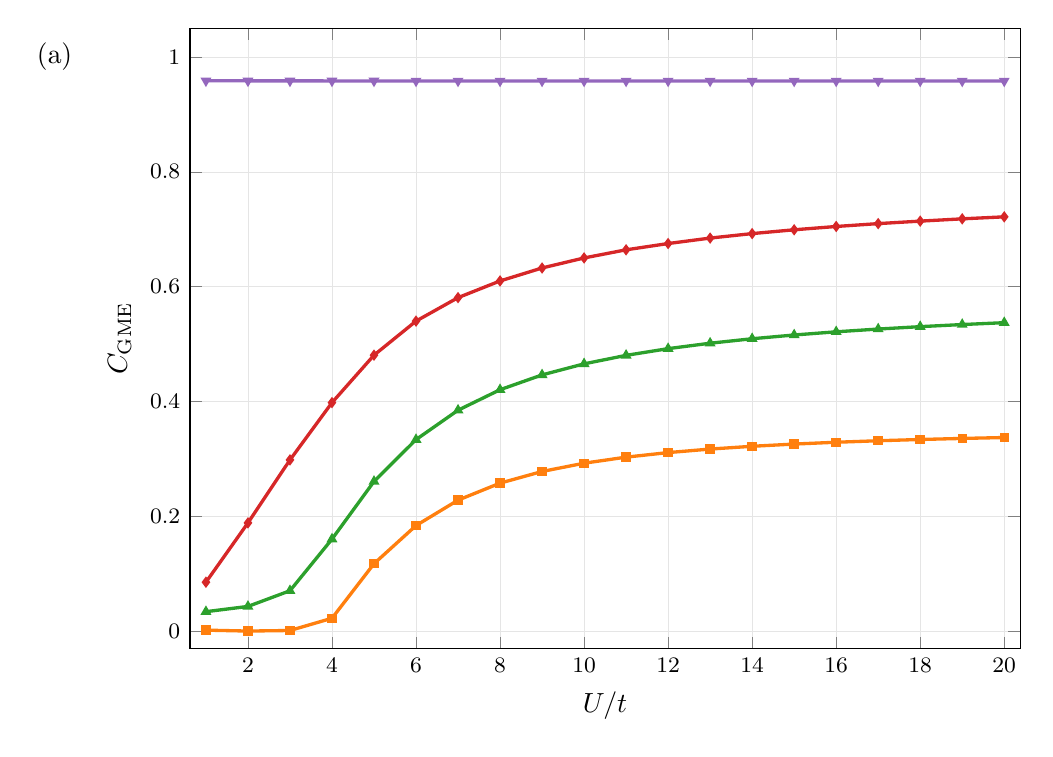
\begin{tikzpicture}
  \begin{axis}[
    width=\columnwidth,
    height=0.78\columnwidth,
    xlabel={$U/t$},
    ylabel={$C_{\mathrm{GME}}$},
    grid=both,
    grid style={line width=.1pt, draw=gray!20},
    tick label style={font=\footnotesize\rmfamily, /pgf/number format/fixed},
    label style={font=\normalsize\rmfamily},
    scaled ticks=false,
    legend style={font=\scriptsize\rmfamily, draw=gray!40, at={(0.5,1.03)}, anchor=south, /tikz/every even column/.append style={column sep=6pt}},
    legend cell align={left},
    legend columns=2,
    ymin=-0.03,
    ymax=1.05,
    xmin=0.62,
    xmax=20.38,
    after end axis/.append code={\node[anchor=east, font=\normalsize\rmfamily] at (axis description cs:-0.13,0.954) {(a)};},
  ]
    \addplot[color=gmeC1, mark=square*, mark size=1.1pt, line width=1.2pt] coordinates {
        (1,0.001781) (2,0.00019) (3,0.001173) (4,0.022499)
        (5,0.117491) (6,0.183917) (7,0.228184) (8,0.25778)
        (9,0.278095) (10,0.292503) (11,0.303051) (12,0.310996)
        (13,0.317128) (14,0.321962) (15,0.325841) (16,0.329003)
        (17,0.331615) (18,0.333798) (19,0.335642) (20,0.337214)
    };
    \addplot[color=gmeC2, mark=triangle*, mark size=1.1pt, line width=1.2pt] coordinates {
        (1,0.033944) (2,0.04309) (3,0.070399) (4,0.160314)
        (5,0.260682) (6,0.333588) (7,0.384779) (8,0.420468)
        (9,0.446274) (10,0.465514) (11,0.480315) (12,0.492004)
        (13,0.501455) (14,0.509252) (15,0.515782) (16,0.521342)
        (17,0.526132) (18,0.530308) (19,0.533977) (20,0.537224)
    };
    \addplot[color=gmeC3, mark=diamond*, mark size=1.1pt, line width=1.2pt] coordinates {
        (1,0.085269) (2,0.188553) (3,0.298219) (4,0.397994)
        (5,0.480619) (6,0.539958) (7,0.580833) (8,0.609883)
        (9,0.632472) (10,0.649929) (11,0.66411) (12,0.675033)
        (13,0.684552) (14,0.692346) (15,0.698997) (16,0.704738)
        (17,0.709743) (18,0.714062) (19,0.718048) (20,0.721531)
    };
    \addplot[color=gmeC4, mark=triangle*, mark size=1.1pt, mark options={rotate=180}, line width=1.2pt] coordinates {
        (1,0.958508) (2,0.958357) (3,0.958276) (4,0.958232)
        (5,0.958209) (6,0.958197) (7,0.95819) (8,0.958186)
        (9,0.958184) (10,0.958182) (11,0.958181) (12,0.958181)
        (13,0.95818) (14,0.95818) (15,0.95818) (16,0.95818)
        (17,0.95818) (18,0.95818) (19,0.958179) (20,0.958179)
    };
  \end{axis}
\end{tikzpicture}
 & % generated by scripts/pkl_to_latex.py
% source PKL : uscan_v1_L6_Ne6_t0p1_mode-uniform_nmin2_solver-gcg_full_es_restarts10_iter300_kmax5_tol1em09_U0.1to5_N21-8081b758e7cc.pkl
% scan type  : uscan
% state      : ex_singlet
% requires   : \usepackage{pgfplots} \pgfplotsset{compat=1.18}
% colours match the matplotlib PDF (tab10 cycle)
\definecolor{gmeC0}{HTML}{1F77B4}
\definecolor{gmeC1}{HTML}{FF7F0E}
\definecolor{gmeC2}{HTML}{2CA02C}
\definecolor{gmeC3}{HTML}{D62728}
\definecolor{gmeC4}{HTML}{9467BD}
\definecolor{gmeC5}{HTML}{8C564B}
\definecolor{gmeC6}{HTML}{E377C2}
\definecolor{gmeC7}{HTML}{17BECF}

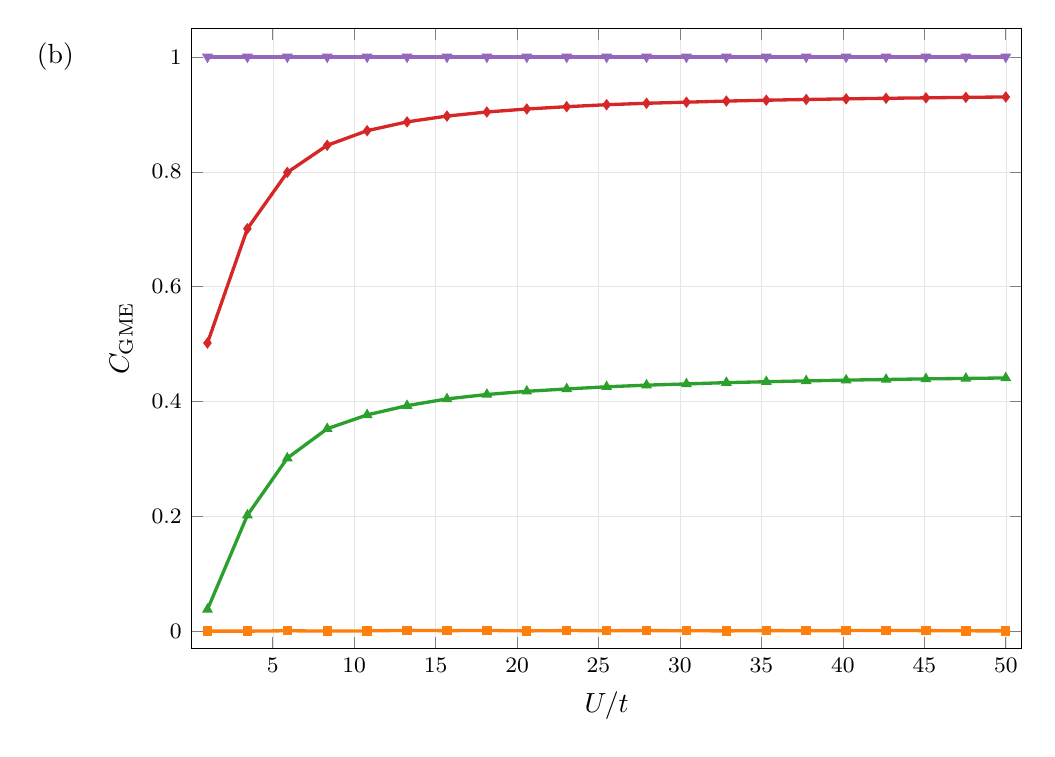
\begin{tikzpicture}
  \begin{axis}[
    width=\columnwidth,
    height=0.78\columnwidth,
    xlabel={$U/t$},
    ylabel={$C_{\mathrm{GME}}$},
    grid=both,
    grid style={line width=.1pt, draw=gray!20},
    tick label style={font=\footnotesize\rmfamily, /pgf/number format/fixed},
    label style={font=\normalsize\rmfamily},
    scaled ticks=false,
    legend style={font=\scriptsize\rmfamily, draw=gray!40, at={(0.5,1.03)}, anchor=south, /tikz/every even column/.append style={column sep=6pt}},
    legend cell align={left},
    legend columns=2,
    ymin=-0.03,
    ymax=1.05,
    xmin=0.02,
    xmax=50.98,
    after end axis/.append code={\node[anchor=east, font=\normalsize\rmfamily] at (axis description cs:-0.13,0.954) {(b)};},
  ]
    \addplot[color=gmeC1, mark=square*, mark size=1.1pt, line width=1.2pt] coordinates {
        (1,0.000076) (3.45,0.000017) (5.9,0.000725) (8.35,0.00013)
        (10.8,0.000477) (13.25,0.001416) (15.7,0.000895) (18.15,0.00125)
        (20.6,0.000461) (23.05,0.001101) (25.5,0.000825) (27.95,0.001059)
        (30.4,0.000767) (32.85,0.000458) (35.3,0.001054) (37.75,0.000683)
        (40.2,0.001019) (42.65,0.001117) (45.1,0.000989) (47.55,0.000616)
        (50,0.000467)
    };
    \addplot[color=gmeC2, mark=triangle*, mark size=1.1pt, line width=1.2pt] coordinates {
        (1,0.037744) (3.45,0.201932) (5.9,0.301295) (8.35,0.352537)
        (10.8,0.376633) (13.25,0.392703) (15.7,0.404476) (18.15,0.412167)
        (20.6,0.417721) (23.05,0.421826) (25.5,0.42556) (27.95,0.428443)
        (30.4,0.430543) (32.85,0.432829) (35.3,0.434396) (37.75,0.435873)
        (40.2,0.437172) (42.65,0.43828) (45.1,0.439383) (47.55,0.440089)
        (50,0.441003)
    };
    \addplot[color=gmeC3, mark=diamond*, mark size=1.1pt, line width=1.2pt] coordinates {
        (1,0.501818) (3.45,0.700882) (5.9,0.798874) (8.35,0.8461)
        (10.8,0.871548) (13.25,0.8869) (15.7,0.897007) (18.15,0.904106)
        (20.6,0.909344) (23.05,0.913356) (25.5,0.916801) (27.95,0.919317)
        (30.4,0.921193) (32.85,0.923135) (35.3,0.924617) (37.75,0.925893)
        (40.2,0.927003) (42.65,0.927977) (45.1,0.928743) (47.55,0.929606)
        (50,0.930293)
    };
    \addplot[color=gmeC4, mark=triangle*, mark size=1.1pt, mark options={rotate=180}, line width=1.2pt] coordinates {
        (1,1) (3.45,1) (5.9,1) (8.35,1)
        (10.8,1) (13.25,1) (15.7,1) (18.15,1)
        (20.6,1) (23.05,1) (25.5,1) (27.95,1)
        (30.4,1) (32.85,1) (35.3,1) (37.75,1)
        (40.2,1) (42.65,1) (45.1,1) (47.55,1)
        (50,1)
    };
  \end{axis}
\end{tikzpicture}
 \\[2pt]
    % generated by scripts/pkl_to_latex.py
% source PKL : uscan_v1_L8_Ne8_t1_mode-uniform_nmin2_solver-gcg_full_restarts8_iter200_kmax4_tol1em09_U1to20_N20-d03a74da789e.pkl
% scan type  : uscan
% state      : gs
% requires   : \usepackage{pgfplots} \pgfplotsset{compat=1.18}
% colours match the matplotlib PDF (tab10 cycle)
\definecolor{gmeC0}{HTML}{1F77B4}
\definecolor{gmeC1}{HTML}{FF7F0E}
\definecolor{gmeC2}{HTML}{2CA02C}
\definecolor{gmeC3}{HTML}{D62728}
\definecolor{gmeC4}{HTML}{9467BD}
\definecolor{gmeC5}{HTML}{8C564B}
\definecolor{gmeC6}{HTML}{E377C2}
\definecolor{gmeC7}{HTML}{17BECF}

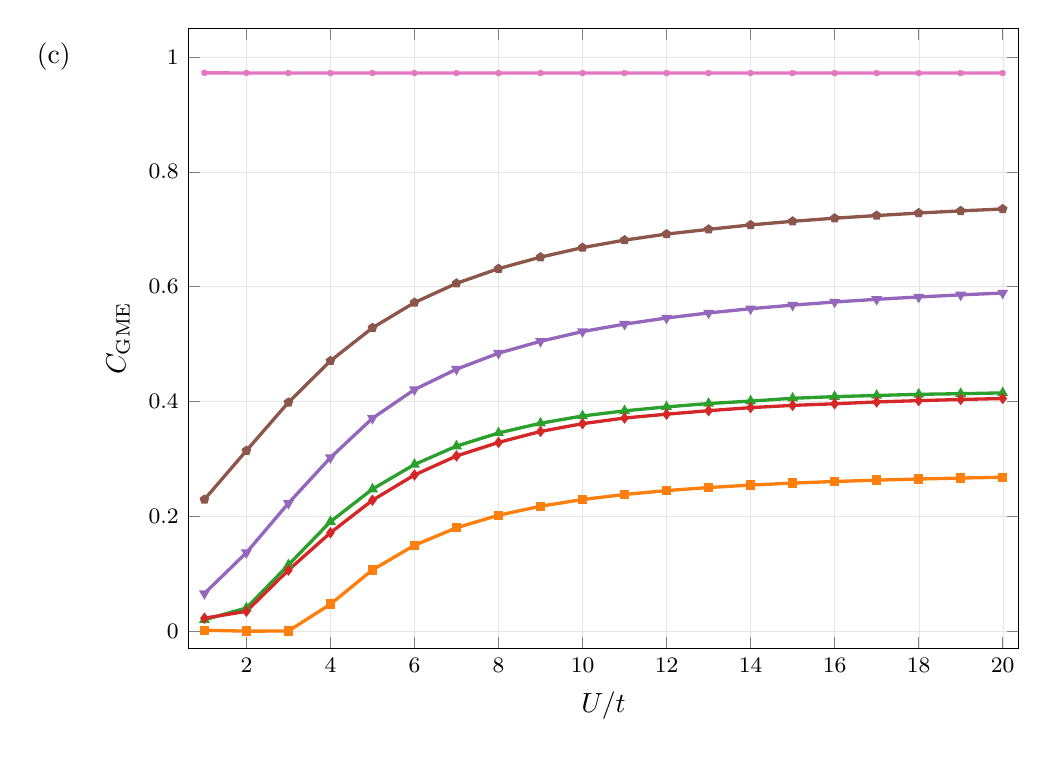
\begin{tikzpicture}
  \begin{axis}[
    width=\columnwidth,
    height=0.78\columnwidth,
    xlabel={$U/t$},
    ylabel={$C_{\mathrm{GME}}$},
    grid=both,
    grid style={line width=.1pt, draw=gray!20},
    tick label style={font=\footnotesize\rmfamily, /pgf/number format/fixed},
    label style={font=\normalsize\rmfamily},
    scaled ticks=false,
    legend style={font=\scriptsize\rmfamily, draw=gray!40, at={(0.5,1.03)}, anchor=south, /tikz/every even column/.append style={column sep=6pt}},
    legend cell align={left},
    legend columns=3,
    ymin=-0.03,
    ymax=1.05,
    xmin=0.62,
    xmax=20.38,
    legend style={at={(0.975,0.035)}, anchor=south east, fill=white},
    after end axis/.append code={\node[anchor=east, font=\normalsize\rmfamily] at (axis description cs:-0.13,0.954) {(c)};},
  ]
    \addplot[color=gmeC1, mark=square*, mark size=1.1pt, line width=1.2pt] coordinates {
        (1,0.001654) (2,0.000044) (3,0.000267) (4,0.046975)
        (5,0.106664) (6,0.149618) (7,0.180102) (8,0.201846)
        (9,0.217602) (10,0.229253) (11,0.238052) (12,0.244832)
        (13,0.250153) (14,0.2544) (15,0.257839) (16,0.260662)
        (17,0.263006) (18,0.264974) (19,0.266641) (20,0.268065)
    };
    \addplot[color=gmeC2, mark=triangle*, mark size=1.1pt, line width=1.2pt] coordinates {
        (1,0.019878) (2,0.040367) (3,0.115422) (4,0.190681)
        (5,0.247387) (6,0.290277) (7,0.322264) (8,0.345138)
        (9,0.362087) (10,0.374752) (11,0.383696) (12,0.390574)
        (13,0.396403) (14,0.400666) (15,0.405558) (16,0.408454)
        (17,0.410431) (18,0.412454) (19,0.413562) (20,0.414928)
    };
    \addplot[color=gmeC3, mark=diamond*, mark size=1.1pt, line width=1.2pt] coordinates {
        (1,0.022574) (2,0.034548) (3,0.106354) (4,0.171385)
        (5,0.228007) (6,0.272007) (7,0.305072) (8,0.328669)
        (9,0.347784) (10,0.36136) (11,0.371204) (12,0.377835)
        (13,0.383977) (14,0.389274) (15,0.393186) (16,0.395985)
        (17,0.39916) (18,0.401473) (19,0.403454) (20,0.405168)
    };
    \addplot[color=gmeC4, mark=triangle*, mark size=1.1pt, mark options={rotate=180}, line width=1.2pt] coordinates {
        (1,0.0656) (2,0.136722) (3,0.222841) (4,0.30224)
        (5,0.370771) (6,0.420742) (7,0.456253) (8,0.484101)
        (9,0.504819) (10,0.521759) (11,0.534672) (12,0.545395)
        (13,0.55418) (14,0.561558) (15,0.567815) (16,0.573218)
        (17,0.577909) (18,0.58201) (19,0.585636) (20,0.588864)
    };
    \addplot[color=gmeC5, mark=pentagon*, mark size=1.1pt, line width=1.2pt] coordinates {
        (1,0.229283) (2,0.314356) (3,0.39842) (4,0.470714)
        (5,0.528206) (6,0.572269) (7,0.605691) (8,0.631318)
        (9,0.651337) (10,0.667933) (11,0.680997) (12,0.691507)
        (13,0.699756) (14,0.707466) (15,0.713749) (16,0.719196)
        (17,0.723774) (18,0.728158) (19,0.731886) (20,0.735217)
    };
    \addplot[color=gmeC6, mark=x, mark size=1.1pt, line width=1.2pt] coordinates {
        (1,0.972294) (2,0.97209) (3,0.971991) (4,0.971943)
        (5,0.971918) (6,0.971905) (7,0.971898) (8,0.971894)
        (9,0.971891) (10,0.97189) (11,0.971889) (12,0.971888)
        (13,0.971888) (14,0.971887) (15,0.971887) (16,0.971887)
        (17,0.971887) (18,0.971887) (19,0.971887) (20,0.971887)
    };
  \end{axis}
\end{tikzpicture}
 & % generated by scripts/pkl_to_latex.py
% source PKL : uscan_v1_L8_Ne8_t0p1_mode-uniform_nmin2_solver-gcg_full_es_restarts10_iter300_kmax5_tol1em09_U0.1to5_N21-8081b758e7cc.pkl
% scan type  : uscan
% state      : ex_singlet
% requires   : \usepackage{pgfplots} \pgfplotsset{compat=1.18}
% colours match the matplotlib PDF (tab10 cycle)
\definecolor{gmeC0}{HTML}{1F77B4}
\definecolor{gmeC1}{HTML}{FF7F0E}
\definecolor{gmeC2}{HTML}{2CA02C}
\definecolor{gmeC3}{HTML}{D62728}
\definecolor{gmeC4}{HTML}{9467BD}
\definecolor{gmeC5}{HTML}{8C564B}
\definecolor{gmeC6}{HTML}{E377C2}
\definecolor{gmeC7}{HTML}{17BECF}

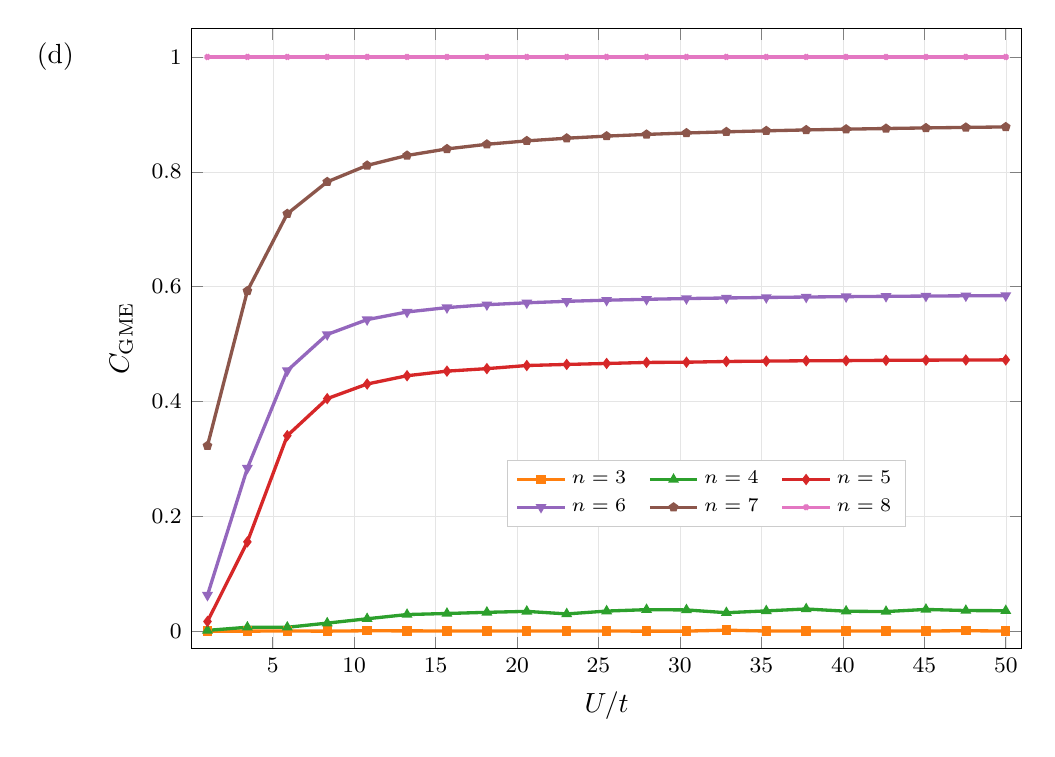
\begin{tikzpicture}
  \begin{axis}[
    width=\columnwidth,
    height=0.78\columnwidth,
    xlabel={$U/t$},
    ylabel={$C_{\mathrm{GME}}$},
    grid=both,
    grid style={line width=.1pt, draw=gray!20},
    tick label style={font=\footnotesize\rmfamily, /pgf/number format/fixed},
    label style={font=\normalsize\rmfamily},
    scaled ticks=false,
    legend style={font=\scriptsize\rmfamily, draw=gray!40, at={(0.5,1.03)}, anchor=south, /tikz/every even column/.append style={column sep=6pt}},
    legend cell align={left},
    legend columns=3,
    ymin=-0.03,
    ymax=1.05,
    xmin=0.02,
    xmax=50.98,
    legend style={at={(0.620,0.250)}, anchor=center, fill=white},
    after end axis/.append code={\node[anchor=east, font=\normalsize\rmfamily] at (axis description cs:-0.13,0.954) {(d)};},
  ]
    \addplot[color=gmeC1, mark=square*, mark size=1.1pt, line width=1.2pt] coordinates {
        (1,0.000027) (3.45,0.00008) (5.9,0.000279) (8.35,0.000053)
        (10.8,0.000729) (13.25,0.000484) (15.7,0.000416) (18.15,0.000175)
        (20.6,0.000142) (23.05,0.00022) (25.5,0.000195) (27.95,0.000112)
        (30.4,0.00013) (32.85,0.001713) (35.3,0.000275) (37.75,0.000342)
        (40.2,0.000365) (42.65,0.000196) (45.1,0.000226) (47.55,0.000816)
        (50,0.000169)
    };
    \addlegendentry{$n=3$}
    \addplot[color=gmeC2, mark=triangle*, mark size=1.1pt, line width=1.2pt] coordinates {
        (1,0.001368) (3.45,0.006876) (5.9,0.006765) (8.35,0.014024)
        (10.8,0.021602) (13.25,0.028958) (15.7,0.030782) (18.15,0.032818)
        (20.6,0.034473) (23.05,0.030047) (25.5,0.035002) (27.95,0.037476)
        (30.4,0.036986) (32.85,0.032141) (35.3,0.035328) (37.75,0.038667)
        (40.2,0.034721) (42.65,0.034156) (45.1,0.037853) (47.55,0.035923)
        (50,0.035619)
    };
    \addlegendentry{$n=4$}
    \addplot[color=gmeC3, mark=diamond*, mark size=1.1pt, line width=1.2pt] coordinates {
        (1,0.016861) (3.45,0.155557) (5.9,0.340486) (8.35,0.404947)
        (10.8,0.430411) (13.25,0.444816) (15.7,0.452822) (18.15,0.457192)
        (20.6,0.46262) (23.05,0.46451) (25.5,0.466183) (27.95,0.467976)
        (30.4,0.468367) (32.85,0.469647) (35.3,0.470287) (37.75,0.470898)
        (40.2,0.471118) (42.65,0.471675) (45.1,0.47198) (47.55,0.472264)
        (50,0.472406)
    };
    \addlegendentry{$n=5$}
    \addplot[color=gmeC4, mark=triangle*, mark size=1.1pt, mark options={rotate=180}, line width=1.2pt] coordinates {
        (1,0.062695) (3.45,0.283926) (5.9,0.453837) (8.35,0.516697)
        (10.8,0.542561) (13.25,0.555869) (15.7,0.563483) (18.15,0.568535)
        (20.6,0.571851) (23.05,0.574409) (25.5,0.576376) (27.95,0.577922)
        (30.4,0.579235) (32.85,0.580236) (35.3,0.581111) (37.75,0.581903)
        (40.2,0.582545) (42.65,0.583098) (45.1,0.583588) (47.55,0.58403)
        (50,0.584425)
    };
    \addlegendentry{$n=6$}
    \addplot[color=gmeC5, mark=pentagon*, mark size=1.1pt, line width=1.2pt] coordinates {
        (1,0.322896) (3.45,0.592553) (5.9,0.726943) (8.35,0.782475)
        (10.8,0.811119) (13.25,0.828414) (15.7,0.839827) (18.15,0.847873)
        (20.6,0.85384) (23.05,0.858461) (25.5,0.862116) (27.95,0.865082)
        (30.4,0.867537) (32.85,0.869599) (35.3,0.871357) (37.75,0.872872)
        (40.2,0.87419) (42.65,0.875349) (45.1,0.876374) (47.55,0.877287)
        (50,0.878107)
    };
    \addlegendentry{$n=7$}
    \addplot[color=gmeC6, mark=x, mark size=1.1pt, line width=1.2pt] coordinates {
        (1,1) (3.45,1) (5.9,1) (8.35,1)
        (10.8,1) (13.25,1) (15.7,1) (18.15,1)
        (20.6,1) (23.05,1) (25.5,1) (27.95,1)
        (30.4,1) (32.85,1) (35.3,1) (37.75,1)
        (40.2,1) (42.65,1) (45.1,1) (47.55,1)
        (50,1)
    };
    \addlegendentry{$n=8$}
  \end{axis}
\end{tikzpicture}

  \end{tabular}
  \caption{Genuine multipartite entanglement concurrence of the spin state extracted from the Hubbard ring at
    half filling ($K=L$), with $V=0$, for different values of the spin number $n$: ground state for (a) $L=6$ and
    (c) $L=8$ sites; first excited singlet for (b) $L=6$ and (d) $L=8$ sites. The same color code for the spin
    number $n$, given in panel (d), is adopted in all panels.}
  \label{fig01}
\end{figure*}

% Alternative: the compiled figure as one PDF (fig12_combined.pdf, made by fig12_combined.tex)
% \begin{figure*}
%   \centering
%   \includegraphics[width=\textwidth]{fig12_combined.pdf}
%   \caption{...}
%   \label{fig01}
% \end{figure*}
